\documentclass[11pt,a4paper]{article}

\usepackage{ctable}
\usepackage[T1]{fontenc}
\usepackage[utf8]{inputenc}
\usepackage{lrec2006}
\usepackage{nicefrac}
\usepackage{apacite}
\usepackage{covington}

\bibliographystyle{apacite}

\let\app=\textsc
\let\oldfrac=\frac
\renewcommand\frac[2]{\mathchoice{\oldfrac{#1}{#2}}{\nicefrac{#1}{#2}}{\nicefrac{#1}{#2}}{\nicefrac{#1}{#2}}}

\title{The Norwegian Dependency Treebank}
\author{Folk}

\frenchspacing

\begin{document}
\maketitle

\section{Introduction}
A syntactic treebank constitutes an important language resource in
establishing a set of natural language processing tools for a
language and may be employed for central tasks such as part-of-speech
tagging and syntactic parsing. For the past decade, dependency
analysis has become an increasingly popular form of syntactic analysis
and has been claimed to strike a balance between a depth of analysis
sufficient for many down-stream applications and accuracy and
efficiency in parsing with these types representations. The CoNLL
shared tasks devoted to dependency parsing and joint syntactic and
semantic parsing,
\cite<see e.g.,>{Niv:Hal:Kub:07,Haj:Cia:Joh:09}, have been instrumental in
establishing a common set of dependency treebanks for a range of
languages such as English, Swedish, Czech and Arabic, \footnote{Note
  that several of the treebanks employed for the shared task were not
  originally dependency treebanks, but rather converted from
  phrase-structure representations.}  thus enabling multilingual evaluation of different systems.  The increased
availability of dependency parsers has spurred down-stream use of
dependency representations in diverse tasks such as Machine Translation \shortcite{Din:Pal:05}, Sentiment Analysis \shortcite{Wil:Wie:Hof:09} and Negation Resolution \shortcite{Lap:Vel:Ovr:12}.

Until recently, no (dependency)
treebank has been publically available for Norwegian.\footnote{Possibly comment on INESS?} Hence,
the progress in parsing and applications described above has not been
possible for Norwegian.  At present, however, the Language Bank,
hosted at the Norwegian National Library, is in the process of
completing a two year project with the aim of producing a dependency
treebank for Norwegian. 

In this paper we present the result of this project, Norwegian Dependency Treebank (NDT), a
syntactic treebank which encompasses treebanks for both variants of
Norwegian (Bokm{\aa}l and Nynorsk)\footnote{On the distinction between
  BM and NN}. In the following, we describe the main annotation
principles employed in the syntactic analysis of the treebank and
discuss the selection of texts. We then go on to describe the
annotation process in some detail. Finally, we present first results
for data-driven dependency parsing of Norwegian.

%311 words

\section{Annotation principles}

%NDT is released in the CoNLL format, a tab-separated table consisting of the following 10 fields: token index, word form, lemma, coarse-grained part-of-speech (POS), fine-grained POS, morphological features, index of head, dependency relation and two fields which are left blank in NDT \cite{Niv:Hal:Kub:07}. 
The texts in NDT are lemmatized, morphologically tagged and annotated with dependency relations and head-dependent graphs. The lemmatization and morphological tagging follow quite closely the Oslo-Bergen Tagger (\cite{Joh:Hag:No:Lyn:2011};OBT), but a few adaptions have been made, notably for spelling variants which do not comply with the official norm for Bokmål and Nynorsk \cite<cf.>{Sol:2013}.


Independent syntactic annotation guidelines have been developed for NDT \cite{Kin:Sol:Eri:2013}. When developing the annotation guidelines, four fundamental principles were taken into consideration: 1. The annotation had to be as linguistically adequate as possible.
%The Norwegian Reference Grammar \cite{Faa:Lie:Van:97} was used as a norm.
2. It had to be possible for annotators to implement the analyzes consistently. 3. As the size of the treebank matters for most potential users, the annotators should be able to annotate relatively quickly.
%, without spending too much time pondering over the correct analysis of specific constructions.
4. It should be relatively easy to make queries for specific constructions, using treebank query tools such as TreeQuery \cite{Paj:Ste:09}. In what remains of this section, we will show examples of how we tried to implement these principles:

\subsection{Adverbials}
In treebanks comparable to NDT, e.g. the Swedish treebank Talbanken \cite{Niv:Nil:Hal:2006}, there are separate dependency relations for different types of adverbials, such as time adverbials, manner adverbials and place adverbials. Some treebanks, e.g. PROIEL \cite{Hau:Joh:Eck:Wel:Her:Mut:2009}, distinguish between adverbials selected by specific predicates, such as motion verbs, and adverbial modifiers which are not obligatory. There may be good linguistic reasons for making such distinctions. However, we found that it would be difficult to do so and at the same time comply with the consistency and time constraints of principle 2 and 3, as there would be frequent borderline cases. Unless the guidelines contained rules which were clear and easy to follow for such cases,chances are high that an annotator would not be able to annotate similar cases in a uniform manner, and inter-annotator consistency would also be difficult to obtain. And even with such rules in place, annotators would spend a considerable amount of time deliberating which dependency relation to choose. We have therefore chosen a more shallow analysis: All adverbials, regardless of type and of whether or not they are selected, receive a uniform dependency relation - ADV.

\subsection{Transitive and intransitive prepositions}
In other cases the pursuit of linguistic adequacy has been given priority. The sentences (\ref{ex:intrans}) and (\ref{ex:trans}) exemplify such a case:

\begin{examples}
\item\label{ex:intrans}
\gll Per setter på CD-en.
Per puts on CD+the
\glt 'Per puts on the CD.'
\glend

\item\label{ex:trans}
\gll Per sitter på stolen.
Per sits on chair+the
\glt 'Per sits on the chair.'
\glend
\end{examples}

In both (\ref{ex:intrans}) and (\ref{ex:trans}) the preposition \emph{på} is followed by a noun. There are, however, strong reasons for analyzing the sentences differently. In (\ref{ex:trans}), the noun is clearly a complement to the preposition: The preposition and the noun are semantically connected, they behave as a single constituent, and the complement retains its position after the preposition if it is pronominalized. In (\ref{ex:intrans}), on the other hand, there is no obvious semantic connection between the preposition and the noun, the two words do not form a constituent together, and if the noun is pronominalized, it usually will precede the preposition. In NDT, the noun in constructions like (\ref{ex:intrans}) would be made dependent on the verb with the dependency relation for direct objects, DOBJ, while in (\ref{ex:trans}) it is made dependent on the preposition with the dependency relation of prepositional complements, PUTFYLL.

Annotators frequently meet preposition-noun sequences which are much less straightforward than in these examples, and they need to deliberate whether one or the other analysis is correct. We have, however, chosen to retain this distinction, to make sure that the analyses are acceptable from a linguistic point of view and also in order to achieve a uniform analysis of sentences such as (\ref{ex:intrans}) and cases where the object noun or pronoun does not follow the intransitive preposition. To ensure consistency and a high annotation speed, the annotation guidelines have a number of syntactic tests which the annotators use to distinguish between the construction \cite[54-56]{Kin:Sol:Eri:2013}.

\subsection{Complementizers}
There is no obvious head-dependent relationship between complementizers and verbs or between functional and lexical heads in general, and there is therefore not a unique answer to how such a relationship should be represented in Dependency Grammar.
%In the original formulation of Dependency Grammar, no dependency relations were indicated between function words and lexical words. Instead, a different, symmetrical relation was used (cf. \cite[361-410]{Tes:65}). In Dependency Grammar treebanks comparable to NDT, no relations apart from assymetrical dependency relations are used. Treebanks vary with respect to the annotation of the complementizer-verbs relations and similar relations between functional and lexical heads.
In NDT, the verb is the head and the complementizer is a dependent on the verb. This choice is first and foremost motivated by the fourth principle stated above: that it should be easy to make queries for specific constructions. In Norwegian, complementizers are frequently dropped, as the following examples show (from NDT):
\begin{examples}
\item\label{ex:medat}
\gll Nå tror lokale myndigheter at bortføringen var nøye planlagt.
now believe local authorities that.comp abduction+the was carefully planned
\glt 'Local authorities now believe that the abduction was carefully planned.'
\glend

\item\label{ex:utenat}
\gll Jeg tror ikke det er tilfeldig.
I believe not it is accidental
\glt 'I don't belive that it is accidental.'
\glend
\end{examples}
 
Clausal complements to verbs such as \emph{tro}, 'believe', occur both with the complementizer \emph{at}, as in (\ref{ex:medat}), and without any complementizer, as in (\ref{ex:utenat}). If the complementizer were the head, the complement clauses in (\ref{ex:medat}) and (\ref{ex:utenat}) would have had different heads, despite their obvious similarities. This, in turn, would make it significantly more difficult to formulate queries in e.g. TreeQuery, that would cover both cases.
%The ability to retrieve constructions through queries has been important in the annotation process, notably in order to find annotation errors, and it will probably also be important to certain users of the treebank.
In NDT, sentences such as (\ref{ex:medat}) and (\ref{ex:utenat}) are analyzed similarly: The (finite) verb of the clausal complement serves as head in both cases, and carry the dependency relation DOBJ (direct object), c.f. figure \ref{figure:medat} and \ref{figure:utenat}. Both will therefore be retrieved through a query for finite verbs with the dependency relation DOBJ.

\begin{figure}[h!]
  \centering
    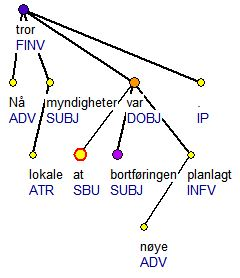
\includegraphics{medat.jpg}
    \caption{Analysis of (\ref{ex:medat})}
    \label{figure:medat}
\end{figure}

\begin{figure}[h!]
  \centering
    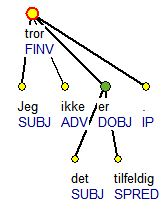
\includegraphics{utenat.jpg}
    \caption{Analysis of (\ref{ex:utenat})}
    \label{figure:utenat}
\end{figure}

% 885 words

\section{Texts}
NDT currently consist of 282 000 tokens of Norwegian Bokmål and 263 000 tokens of Norwegian Nynorsk, but these numbers will grow somewhat until the end of the project period in January 2014. Comparable treebanks such as the Prague Dependency Treebank and the TIGER treebank, contain mainly newspaper text \cite{Boh:Haj:Hla:2003,Bra:2004}. Other treebanks, e.g. Penn Treebank and Talbanken \cite{Mar:San:Mar:93,Niv:Nil:Hal:2006}, however, also contain texts from other sources, such as factual prose, fiction and text in a more colloquial style style. Since newspaper text is frequently used for various NLT tasks and also easily available, we chose to use mostly newspaper text in the NDT, but we added small amounts of text from government reports, parliament transcripts and more colloquial texts from blogs. In the final version of NDT, it will be possible to extract specific genres of text.

\ctable[botcap,
    caption={Distribution of texts in the treebanks},
    label=tb:distribution,
    mincapwidth=\columnwidth
]{lr@{\%}}{}{
        \FL
        Source & \multicolumn{1}{c}{Fraction} \ML
Newspaper text & 84 \NN
Government reports & 6 \NN
Parliament transcripts & 4 \NN
Blogs & 6
        \LL
    }

% 138 words 

\section{Annotation process}
\subsection{Annotators}
All texts in the treebank have been manually annotated by trained linguists. A few of the texts have been syntactically annotated by two annotators, to ensure consistency (cf. \ref{sc:inter-a}). In order to speed up the annotation process, we chose to preprocess the texts using tools already available at the University of Oslo. This process will be described in more detail below.

\subsection{Preprocessing and work flow}
As is standard practice when annotating syntactic corpora, the texts to be
annotated are automatically PoS tagged and syntactically parsed before being
annotated, an approach which has been shown to be both fast and yielding
high quality annotation \cite{Mar:San:Mar:93,For:Sag:10,Skjaerholt:13}.
After tokenization, the texts to be annotated are first tagged using OBT, and
a HMM-based overlay \cite{Joh:Hag:No:Lyn:2011} is used to disambiguate any
tokens with more than one tag remaining. The morphological annotation is then
checked and corrected by an annotator using a web interface made for this
particular task \cite{Lyn:13}. The corrected morphological annotations are
then preprocessed by a dependency parser and imported into \app{TrEd}, the
annotation tool developed for the Prague Dependency Treebank, which is used to
correct the output of the syntactic preprocessing and create the final
treebank.

Since there were no publicly available dependency corpora at the start of this
project, training a data-driven dependency parser such as MaltParser was
impossible. Therefore, the initial syntactic preprocessor was created using
the syntactic module of OBT, which while it does not create a hierarchical
structure, does provide some information about heads. On top of this we built
a small set of rules in the CG-3 framework (<ref Bick>) to build proper
syntactic structures. This preprocessor was evaluated to get about 80\% of
heads correct (unlabelled attachment) and both head and label (labelled
attachment) correct in 72--74\% of cases, as shown in Table \ref{tbl:parsers}.

The first statistical parser trained on the corpus is that of
\citeA{Skj:Ovr:12}, which was later used in inter-annotator agreement
experiments of \citeA{Skjaerholt:13}, reported to reach a labelled accuracy of
84\% and an unlabelled accuracy of 87\%. Based on this, an improved parser was
trained which obtains an unlabelled accuracy of nearly 90\% and labelled
accuracy of 87\%. Note that these results are not entirely comparable as they
are evaluated on different corpora, but given the important differences in
performance, the improved parsers are clearly better. In particular, the
difference between the CG parser and that of \citeA{Skj:Ovr:12} resulted in
significant increases in annotator productivity \cite{Skjaerholt:13}.

\ctable[botcap,
    caption={Preprocessor accuracies. Unlabeled (UAS) and Labeled (LAS)
    attachment scores, and label accuracies (Labels).},
    label=tbl:parsers,
    mincapwidth=\columnwidth,
    notespar,
]{l@{~(}c@{)\hspace{1em}}r@{.}lr@{.}lr@{.}l}{}{
        \FL
\multicolumn{2}{c}{Parser} & \multicolumn{2}{c@{\hspace{1em}}}{UAS} & \multicolumn{2}{c@{\hspace{1em}}}{LAS} & \multicolumn{2}{c@{\hspace{0.5em}}}{Labels} \ML
CG & BM            & 79&39\% & 72&45\% & 82&10\% \NN
CG & NN            & 80&16\% & 74&76\% & 84&84\% \NN
S \& Ø (2012) & BM & 87&54\% & 84&63\% & 89&63\% \NN
Final & BM         & 89&89\% & 87&57\% & 91&70\% \NN
Final & NN         & 89&66\% & 87&50\% & 91&76\%
        \LL
    }

% Need to set a standard evaluation corpus to properly compare the different
% preprocessors. Which has to be different from the training material of *all*
% the MaltParsers (most important in that respect is the most recent one from
% PE.
%
% Given this, it might make sense to merge or at least connect this part to
% the section of dependency parsing.

\subsection{Inter-annotator agreement}
\label{sc:inter-a}
To validate the consistency of the annotations produced by the different
annotators, a set of experiments quantifying inter-annotator agreement were
performed \cite{Skjaerholt:13}. As is common practice in the field of
syntactic annotation \cite{Civit:ea:03,Brants:00,Bra:Han:02,Hajic:04}, the
simple agreement measures labelled and unlabelled attachment accuracy were
used. The reason for using an uncorrected measure rather than a
chance-corrected measure such as $\kappa$ or $\pi$ is that these measures are
not directly applicable to the task of syntactic annotation.

\ctable[botcap,
    caption={Inter-annotator agreement using different preprocessors},
    label=tb:agreement,
    mincapwidth=\columnwidth,
]{lcr@{.}lr@{.}l}{}{
        \FL
\multicolumn{2}{c}{Preprocessor ($\frac{\mathrm{UAS}}{\mathrm{LAS}}$)} & \multicolumn{2}{c@{\hspace{1em}}}{UAS} & \multicolumn{2}{c@{\hspace{0.5em}}}{LAS} \ML
Danish    & ($\frac{72.5\%}{39.2\%}$) & 96&3\% & 94&0\% \NN
Swedish   & ($\frac{79.1\%}{68.7\%}$) & 96&1\% & 94&4\% \NN
Norwegian & ($\frac{87.5\%}{84.6\%}$) & 96&8\% & 95&3\%
        \LL
    }

Table \ref{tb:agreement} shows the labelled and unlabelled attachments for
three different preprocessors, all three taken from those trained by
\citeA{Skj:Ovr:12}. The first two preprocessors, labelled Danish and Swedish
use cross-lingual parsers adapdted from the Danish Dependency Treebank
\cite{Kromann:03} and Talbanken05 \cite{Niv:Nil:Hal:2006}, respectively. To
create these parsers, the PoS and dependency relation tagsets of the source
treebanks were mapped into the corresponding tagsets used by the NDT and
differing opinions on head selection were accounted for by transforming the
relevant constructions in the sources into the representations licensed by the
NDT guidelines. The Danish parser is delexicalised (that is, the Danish
word-forms have been removed from the training corpus) while the Swedish
parser was trained on a lexicalised corpus (no spelling normalisation was
performed).

As is clear from the data in the table, inter-annotator agreement is uniformly
high, regardless of the quality of the parser used for preprocessing.
Agreement on heads as measured by unlabelled attachment does not appear to
change appreciably as a function of preprocessor performance, but labelled
attachment does increase somewhat, from 94.0\% using the Danish parser to
95.3\% with the Norwegian parser. These results are comparable to those
reported for the German NEGRA \cite<92.4\% labelled $F_1$,>{Brants:00} and
TIGER \cite<93.9\% labelled $F_1$,>{Bra:Han:02} treebanks and the Spanish
Cat3LB treebank \cite<86.9\% labelled bracket precision,>{Civit:ea:03}.

\section{Dependency parsing}
%TO-DO: note that final version of the paper will contain results from the final version of the treebank
An important aspect of treebank annotation relates to its \emph{parsability},
i.e. the quality of syntactic parsers that can be acquired based on
the treebank data.  In order to investigate the parser quality we can
expect from NDT, we have evaluated three state-of-the-art dependency
parsers on the material: Maltparser \shortcite{Niv:Hal:Nil:06},
MST-parser \shortcite{McD:Per:Rib:Haj:05} and the parser of
\citeA{Boh:Niv:12}. These implement different parsing strategies: Maltparser is a transition-based parser with local learning and greedy search, MST is a graph-based dependency parser implementing global, near-exhaustive search and the \citeA{Boh:Niv:12} parser is a transition-based dependency parser with joint tagger that
implements global learning and a beam search for non-projective labeled
dependency parsing. 
This latter parser has recently outperformed pipeline systems (such as the
Malt and MST parsers) both in terms of tagging and parsing accuracy for
typologically diverse languages such as Chinese, English, and German. 
For Maltparser, we trained two versions of the
parser: one version with default settings and one optimized version,
where the parser settings was optimized using the MaltOptimizer
software \shortcite{Bal:Niv:12}. Both the MST and \citeA{Boh:Niv:12}
parsers were trained using default settings.

For these experiments, both portions of the treebank (Bokm{\aa}l and
Nynorsk) were split into 80-10-10 train, development and test sets.
Standard evaluation metrics in dependency parsing are unlabeled and
labeled attachment scores (UAS, LAS; implemented by the CoNLL
\textsf{eval.pl} scorer).  These measure the proportion of tokens
which are correctly attached to their head token and, for LAS,
furthermore have been assigned the correct dependency label.


%121 words


\ctable[botcap,
    caption={Dependency parsing results for NDT},
    label=tb:parsing
]{lll@{\hspace{2em}}ll}{}{
        \FL
    & \multicolumn{2}{c@{\hspace{2em}}}{Bokm{\aa}l (BM)} & \multicolumn{2}{c}{Nynorsk (NN)} \NN
    & UAS & LAS  & UAS & LAS \ML
Malt default & 88.27 & 85.03 & 87.54 & 83.82 \NN
Malt optimized & 92.19 & 89.82 & 91.57 & 88.98 \NN
MST  & 91.69 & 88.26 & 91.54 & 87.80 \NN
Bohnet\&Nivre & 92.94 & 90.56 & 92.78 & 90.18 
        \LL
    }

Table \ref{tb:parsing} presents the dependency parsing results
obtained for NDT. We find that the \citeA{Boh:Niv:12} parser
outperforms the other parsers and obtains labeled accuracy scores of
90.6 and 90.2 for the BM and NN treebanks, respectively.
The optimized Maltparser model performs onlys slightly lower, at 89.8 and 89.0. 

\clearpage
\bibliography{ndt}

\end{document}
